\documentclass[10pt,twocolumn,letterpaper]{article}

\usepackage{cvpr}
\usepackage{times}
\usepackage{epsfig}
\usepackage{graphicx}
\usepackage{amsmath}
\usepackage{amssymb}
\usepackage{appendix}

% Include other packages here, before hyperref.

% If you comment hyperref and then uncomment it, you should delete
% egpaper.aux before re-running latex.  (Or just hit 'q' on the first latex
% run, let it finish, and you should be clear).
\usepackage[breaklinks=true,bookmarks=false]{hyperref}

\cvprfinalcopy % *** Uncomment this line for the final submission

\def\cvprPaperID{****} % *** Enter the CVPR Paper ID here
\def\httilde{\mbox{\tt\raisebox{-.5ex}{\symbol{126}}}}

% Pages are numbered in submission mode, and unnumbered in camera-ready
%\ifcvprfinal\pagestyle{empty}\fi
\setcounter{page}{1}
\begin{document}

%%%%%%%%% TITLE
\title{Face Tracking System with Emotion Detection and Face Matching}

\author{Yaxi Lei\\
Brown University\\
{\tt\small yaxi\_lei1@brown.edu}
% For a paper whose authors are all at the same institution,
% omit the following lines up until the closing ``}''.
% Additional authors and addresses can be added with ``\and'',
% just like the second author.
% To save space, use either the email address or home page, not both
\and
Qiran Gong\\
Brown University\\
{\tt\small qiran\_gong@brown.edu}
\and
Da Huo\\
Brown University\\
{\tt\small da\_huo@brown.edu}
}

\maketitle
%\thispagestyle{empty}

%%%%%%%%% ABSTRACT
\begin{abstract}
   Efficient face tracking system has became an essential application in modern society which has many use cases including security surveillance, identity checking, and many other purposes. In this project, we propose to implement a real-time face tracking system that includes emotion detection and face matching features. Both features can be used under many situations. Our system achieves efficient real-time multi-face detection with emotion labels. 
\end{abstract}

%%%%%%%%% BODY TEXT
\section{Introduction}
Face detection is widely used in many modern applications. For this project, we aim to explore some of the state-of-the-art face detection techniques while incorporating our own models to build a real-time face tracking system. The systems consists of 3 main parts -- face detection, face matching, and emotion detection. For the face detection part, our original plan was to implement the Multi-task Cascaded Convolutional Networks \cite{MTCNN}. However, while implementing MTCNN\cite{MTCNN}, our model suffers a poor performance and we realized that it is very hard for us to out-perform the existing MTCNN\cite{MTCNN} libraries. Therefore, we decides to use existing MTCNN libraries for the face detection part and build new features upon face detection. For the face matching part of this project, the goal is to detect whether a face captured by MTCNN\cite{MTCNN} exists in our database. We built a deep convolutional neural network which takes two images of face as input and outputs whether these two images are the face of the same person. Section ~\ref{sec:faceMatching} describes this part in detail. For the emotion detection part of this project, the goal is to detect the emotion of the captured face. We built a Convolutional Neural Network that takes a captured face image as input and classifies it into one of 7 emotions {Angry, Disgust, Fear, Happy, Sad, Surprise, Neutral}. We used the FER-2013 dataset \cite{Goodfeli-et-al-2013} to train our model and achieved a decent result. section ~\ref{sec:emotion} describes this part in detail.
\section{Related Work}

Similar to siamese networks\cite{chopra2005learning}, in face matching part, we take two face images as model's input. Based on siamese networks, our model can combine feature extraction with similarity measurements and learn parameters, which forms an end-to-end framework. For the feature extraction part, many different deep network architecture have been used to great success in computer vision community, like VGG16\cite{simonyan2014very}, ResNet-50\cite{he2016deep}, etc. Both VGG16 and ResNet-50 introduce a concept: block. They treat multiple convolution layers as a block and stack blocks as their neural networks. Additionally, ResNet-50 has a key concept: residual. Residual is actually the output from last block and ResNet combines outputs from different blocks to avoid gradient vanishing problem. However, networks mentioned above are complicated and  all trained on large scale dataset, for example: ImageNet\cite{deng2009imagenet}. Given that our dataset scale is relative small, we thus take a relative simple network, which is similar to LeNet\cite{lecun1998gradient}. Different from LeNet, we additionally add one convolution layer and remove max-pooling between convolution layers except the last one. The reason why we change LeNet like that is we have used MTCNN\cite{MTCNN} to remove background information and we hope to keep as much information as we can extracted from people's faces. 
\section{Method}
\subsection{Face Matching}
\label{sec:faceMatching}
The goal of facial Matching is to retrieve whether new faces can find matches in the database. Therefore, the problem can be summarized as calculating the similarity between pictures. 
% MTCNN 记得搞reference 好的
Before model training, we first use MTCNN\cite{MTCNN} to extract people's faces from pictures. This step of data preprocessing is to filter some useless background information. After face extraction, we stack all faces together and generate random pairs of index. Labels are binary, meaning similar or not for each pair of faces. To overcome data unbalancing problem, we take down sampling method in machine learning. 

Then, our method uses pair-wise training, which can be divided into two parts: feature extraction and similarity measurement. For the first part, we uses 3-layer CNNs and 2 Dense layers and add a max-pooling layer to filter some redundant information. Because we hope to keep original information from faces, we only add one pooling layer. To avoid overfitting problems, drop out layers are added between dense layers. For the second part, we simply concatenate features extracted from above-mentioned CNNs architecture, and pass it into dense layers to do the binary classification. The whole model structure is shown in Figure 1\label{fig:result1}. 
\begin{figure}[h]
    \centering
    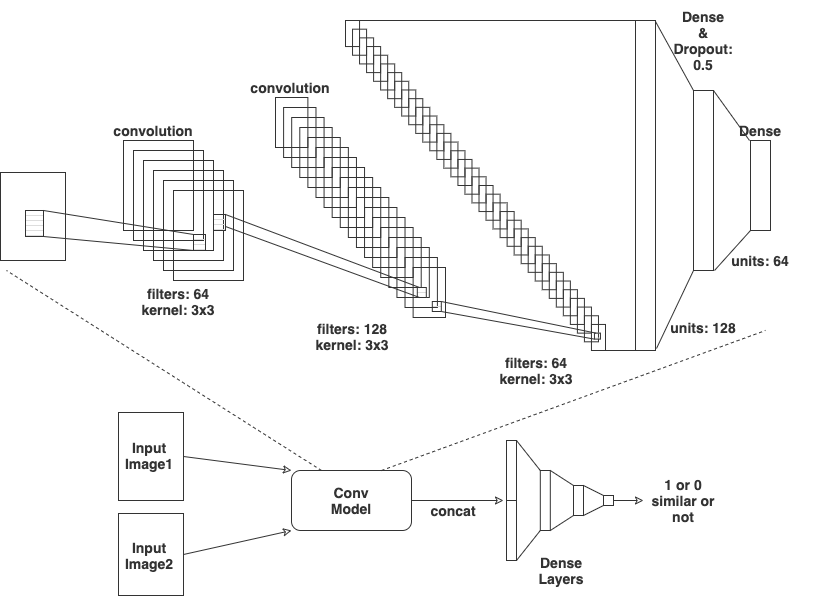
\includegraphics[width=5cm]{face recognition.png}
    \caption{facial matching model architecture}
    \label{fig:result1}
\end{figure}
\subsection{Emotion Detection}
\label{sec:emotion}
For this part, we built a Convolutional Neural Network to classify the captured face image into one of 7 emotions {Angry, Disgust, Fear, Happy, Sad, Surprise, Neutral} and we trained our network using the Facial Expression Recognition 2013 (FER-2013) Dataset \cite{Goodfeli-et-al-2013} which contains 35887 $48 * 48$ size images. Among those 37887 images, we used $28709$ images as our training data, 3589 images as validation data, and 3589 images as testing data.  The training, validation and testing data ratio is roughly about $8:1:1$. 

\\
As for our network architecture, initially we started with a fairly complex model structure which contains 15 layers. The architecture first have 12 convolutional layers and a max-pooling layer for every three convolutional layers. We used relu as our activation for all the convolutional layers. We also have 3 dense layers with relu activation after the convolutional layers. Figure ~\ref{fig:complex_model} shows the detailed model architecture of our initial model. 
\begin{figure}[h]
    \centering
    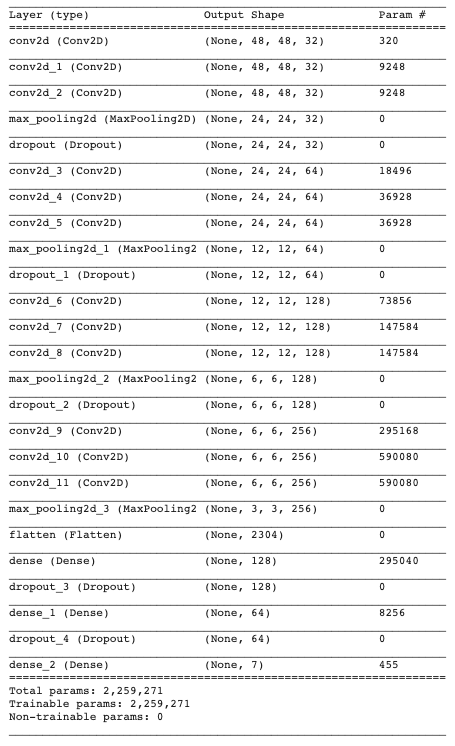
\includegraphics[width=7cm]{complex_model.png}
    \caption{Initial Emotion Detection Model Architecture}
    \label{fig:complex_model}
\end{figure}
However, this model does not perform as good as we expected it to be. The model stuck on about $60\%$ accuracy and most importantly, the model will predict ``Angry" for the most of the time. The reason for this could be that the model is too complex given the limited data we have and it overfits too much on the training dataset. Thus, we switched to a simpler model structure. 

\\
Our new model structure consists a total of 7 layers which includes 4 convolutional layers and 3 dense layers. We used relu activation for all convolutional and dense layers and max-pooling in between of every convolutional layers. Figure ~\ref{fig:simple_model} shows a detailed model structure of our new model.
\begin{figure}[h]
    \centering
    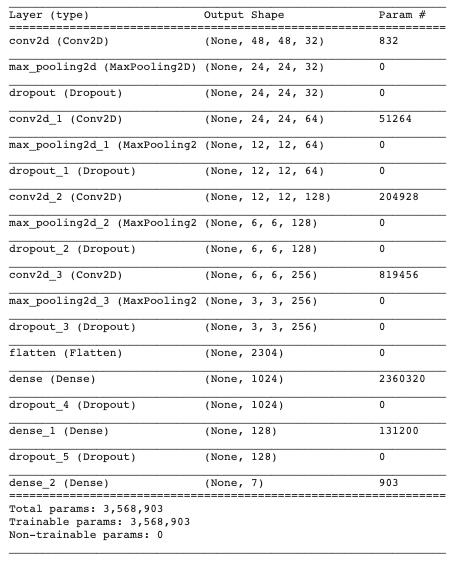
\includegraphics[width=7cm]{simple_model.png}
    \caption{New Emotion Detection Model Architecture}
    \label{fig:simple_model}
\end{figure}

Initially we trained this model with a dense layer of size $128$ and the model gives poor performance every time. After extensive testing and research, we found out that it could be the dense layer size is too small to catch all the features captured by convolutional layers. After we increase the dense layer size to $1024$, the model starts to give decent results.

\\
Although our new model gives a decent result, the model suffers from limited training data. To deal with this situation, we augmented our training data during the training process. We augumented the training data with the following parameters
\begin{verbatim}
    datagen = ImageDataGenerator(
    rescale=1./255,
    width_shift_range=0.1,
    height_shift_range=0.1,
    zoom_range=0.1
    )
\end{verbatim}



\section{Results}
\subsection{Face Matching}
There are four concepts in statistics: true positive (TP), true negative (TN), false positive (FP) and false negative (FN).
A true positive is an outcome where the model correctly predicts the positive class. Similarly, a true negative is an outcome where the model correctly predicts the negative class. A false positive is an outcome where the model incorrectly predicts the positive class. To better define f1 score, we first introduce another two terms: precision and recall. Precision measures model's performance on true samples, which is defined as $\frac{TP}{TP+FP}$. Recall measures model's capability of finding correct predictions on true samples, which can be defined as $\frac{TP}{TP+FN}$.

Considering that only using accuracy might cause bias on model's performance, thus for the face matching part, we choose accuracy and f1 score as evaluation metric. Accuracy is used to evaluate the closeness between prediction and labels, which is defined as $\frac{TP+TN}{TP+TN+FP+FN}$. F1 score is defined as $2 \cdot \frac{precision \cdot recall}{precision + recall}$ Our dataset is divided into training set, validation set and testing set by 8:1:1. After 100 training epochs, the accuracy and f1 score of our model can reach 0.9559 and 0.9549 respectively. 

\subsection{Emotion Detection}
To evaluate our emotion detection model, we used the model accuracy which can be calculated as
\begin{equation}
    Accuracy = \frac{TP}{TP + FN}
\end{equation}
where TP is True Positive and FN is false negative. 

\\

For our initial model which has a more complex structure, the model's validation accuracy and training accuracy can be view in figure ~\ref{fig:complex_model_result}
\begin{figure}[h]
    \centering
    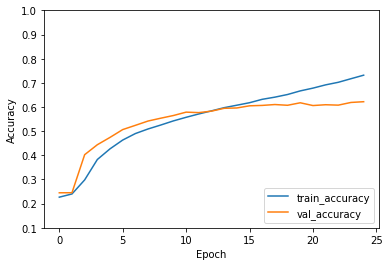
\includegraphics[width=7cm]{complex_model_result.png}
    \caption{Initial Emotion Detection Model Accuracy}
    \label{fig:complex_model_result}
\end{figure}

As we can see from the figure, the model starts to overfit around $60\%$ accuracy. We tried to tune the model with varies hyperparameters and the best we can get is to start to overfit around $60\%$ accuracy. For this model, the model's can reach more than $90\%$ training accuracy with its complex architecture. However, it performs poorly on the testing dataset and validation dataset as it tends to always predict ``Angry". 

\\
For our second model which is the simpler one, the model's validation accuracy and training accuracy can be view in figure ~\ref{fig:simple_model_result}
\begin{figure}[h]
    \centering
    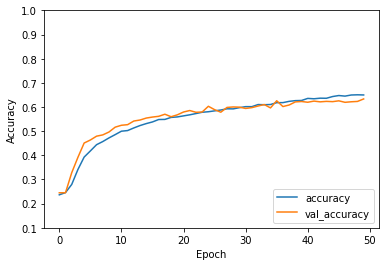
\includegraphics[width=7cm]{simple_model_result.png}
    \caption{Second Emotion Detection Model Accuracy}
    \label{fig:simple_model_result}
\end{figure}

As we can see from the figure, both the model's training accuracy and validation accuracy comes to a convergence at around $63\%$ accuracy. The reason for this could be that given it's simple model structure, this is the best that this architecture can learn unlike our first model which can overfit to a high training accuracy. In addition, unlike the first model, this model gives a more reasonable prediction as it does not rely on predicting ``Angry". It gives a more evenly distributed prediction and is particularly good at Happy, Surprise, Sad, and Angry emotions. Thus, we used this model in our final implementation of the face tracking system.  

\subsection{Integrated System}
As a final result, our system is capable of capturing multiple faces in a given video frame, give each face a emotion label, and match the face with a potential face database in real time. When running the program, an example of the video window is shown as figure ~\ref{fig:face}
\begin{figure}[h]
    \centering
    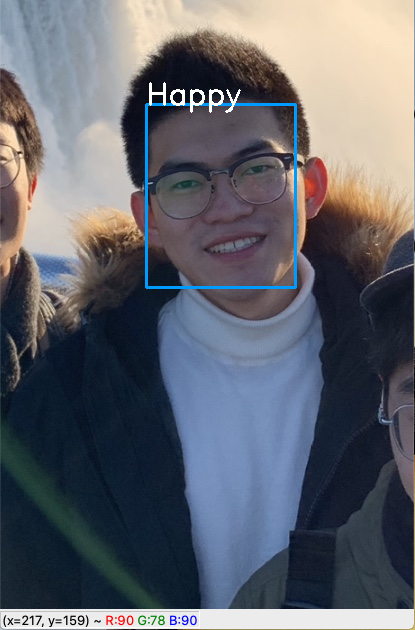
\includegraphics[width=6cm]{face.png}
    \caption{Program Example}
    \label{fig:face}
\end{figure}

\section{Instructions on Running Our System}
To run our system for a demo,
\begin{enumerate}
    \item Clone the project repo
    \begin{verbatim}
        git clone https://github.com/
        MangoManGeek/CV_final_project
    \end{verbatim}
    
    \item install required packages from requirements.txt
    \item run csci1430-final.py
    \begin{verbatim}
        python3 csci1430_final.py
    \end{verbatim}
\end{enumerate}

\section{Conclusion}
In this project, our group was able to build a real-time face tracking system with emotion detection and face matching features using various Computer Vision and Deep learning techniques. We believe this system can be useful in many modern applications. However, processing image frames is a computation heavy task. We have to slow the frame rate in our current implementation in order to achieve real-time processing. Thus, our future work is to come up with a more efficient implementation or even model structure to provide a high frame per second rate.  



%%%%% REFERENCES
\bibliographystyle{unsrt}
\bibliography{reference}

\newpage
\appendixpage
\section{Team Member Contributions}
\textbf{Yaxi Lei:} MTCNN model build and research; Overall system integration with all features; Presentation
\\

\textbf{Qiran Gong:} Face Matching model build and research; Writing report
\\

\textbf{Da Huo:} Emotion Detection model build and research; Writing report
\end{document}
